\section{Methods}

We use two atmospheric models to estimate the atmospheric changes: the first is a simple one-dimensional model of a convective boundary layer, and the second is a complex three-dimensional regional climate model.  Because of their differing levels of complexity, these models have complementary strengths and weaknesses.  The simple model isolates the central physical processes of land surface energy partitioning and entrainment of free tropospheric air; however, the simple model neglects secondary but important processes such as lateral advection, topographic effects on flow, and radiation change.  The complex model, on the other hand, includes these and many other processes and can thus represent spatial heterogeneity and unanticipated feedbacks; however, the inclusion of so many processes can obscure the connection between stomatal dynamics and temperature and humidity changes.  By using both models, we test the robustness of the stomatal effects and explore both the central processes and the complex implications.

In both models, we use the stomatal response parameters for soil moisture and $VPD$ derived in the previous chapter to calculate stomatal conductance and thus latent heat flux.  Tests with each model are conducted over a range of soil moisture values and synoptic conditions typical of August in the northern California Coast Range.  We quantify the differences in surface temperature, near-surface air temperature, boundary layer depth, and near-surface humidity between a hypothetical all-Douglas-fir forest and a hypothetical all-Pacific-madrone forest.

We account for variability of radiative and synoptic forcing differently in each model.  In the simple model, where the response to variability in radiation and free troposphere inputs is more linear, the model simulation period is one day, using average radiation forcing for mid-August; this one-day simulation is repeated for three sets of free troposphere conditions, to characterize the sensitivity to synoptic forcing.  In the complex model, where the response to variability in radiation and free troposphere inputs is nonlinear, we instead run the model for a longer period (two weeks) with evolving radiative and synoptic (lateral boundary) inputs, and we average the the model output over this variability in inputs.

Two soil moisture quantities are used in this chapter.  The first, volumetric soil moisture ($\theta_{vol}$), represents the volume of water per total volume of soil (m$^3$/m$^3$) and is used in the complex model's land surface model.  The second, relative soil moisture ($\theta_{rel}$), equals the actual volumetric soil moisture divided by the volumetric soil moisture at saturation ($\theta_{max}$):
\begin{equation}
\theta_{rel} = \theta_{vol} / \theta_{max}.
\end{equation}
Relative soil moisture is used in Chapter \ref{c.sapflow} and in this chapter's simple model.  Volumetric soil moisture is used in this chapter's comprehensive model.

\subsection{1-D model}
The 1-D model [\cite{tennekes1981basic}; \cite{garratt1994atmospheric}; \cite{Siqueira:2009qf}] simulates the evolution of boundary layer height, potential temperature, and humidity, given surface fluxes and free troposphere conditions.  In the real daytime atmospheric boundary layer (Figure \ref{fig:BL_schematic}(a)), potential temperature ($\Theta$, K) and specific humidity ($Q$, g/kg) decrease rapidly with height through the surface layer, are uniform with height in the mixed layer, and transition toward their free-tropospheric profiles in an entrainment zone at the top of the boundary layer.  This structure is simplified in the 1-D model (Figure \ref{fig:BL_schematic}(b)): the boundary layer is assumed to be well mixed, with uniform $\Theta$ and $Q$, and to be capped by a temperature inversion represented by a step change.  Because the model is 1-D, it assumes horizontal homogeneity, meaning no lateral variation in surface fluxes or properties and no net horizontal advection.

\begin{figure}[here]
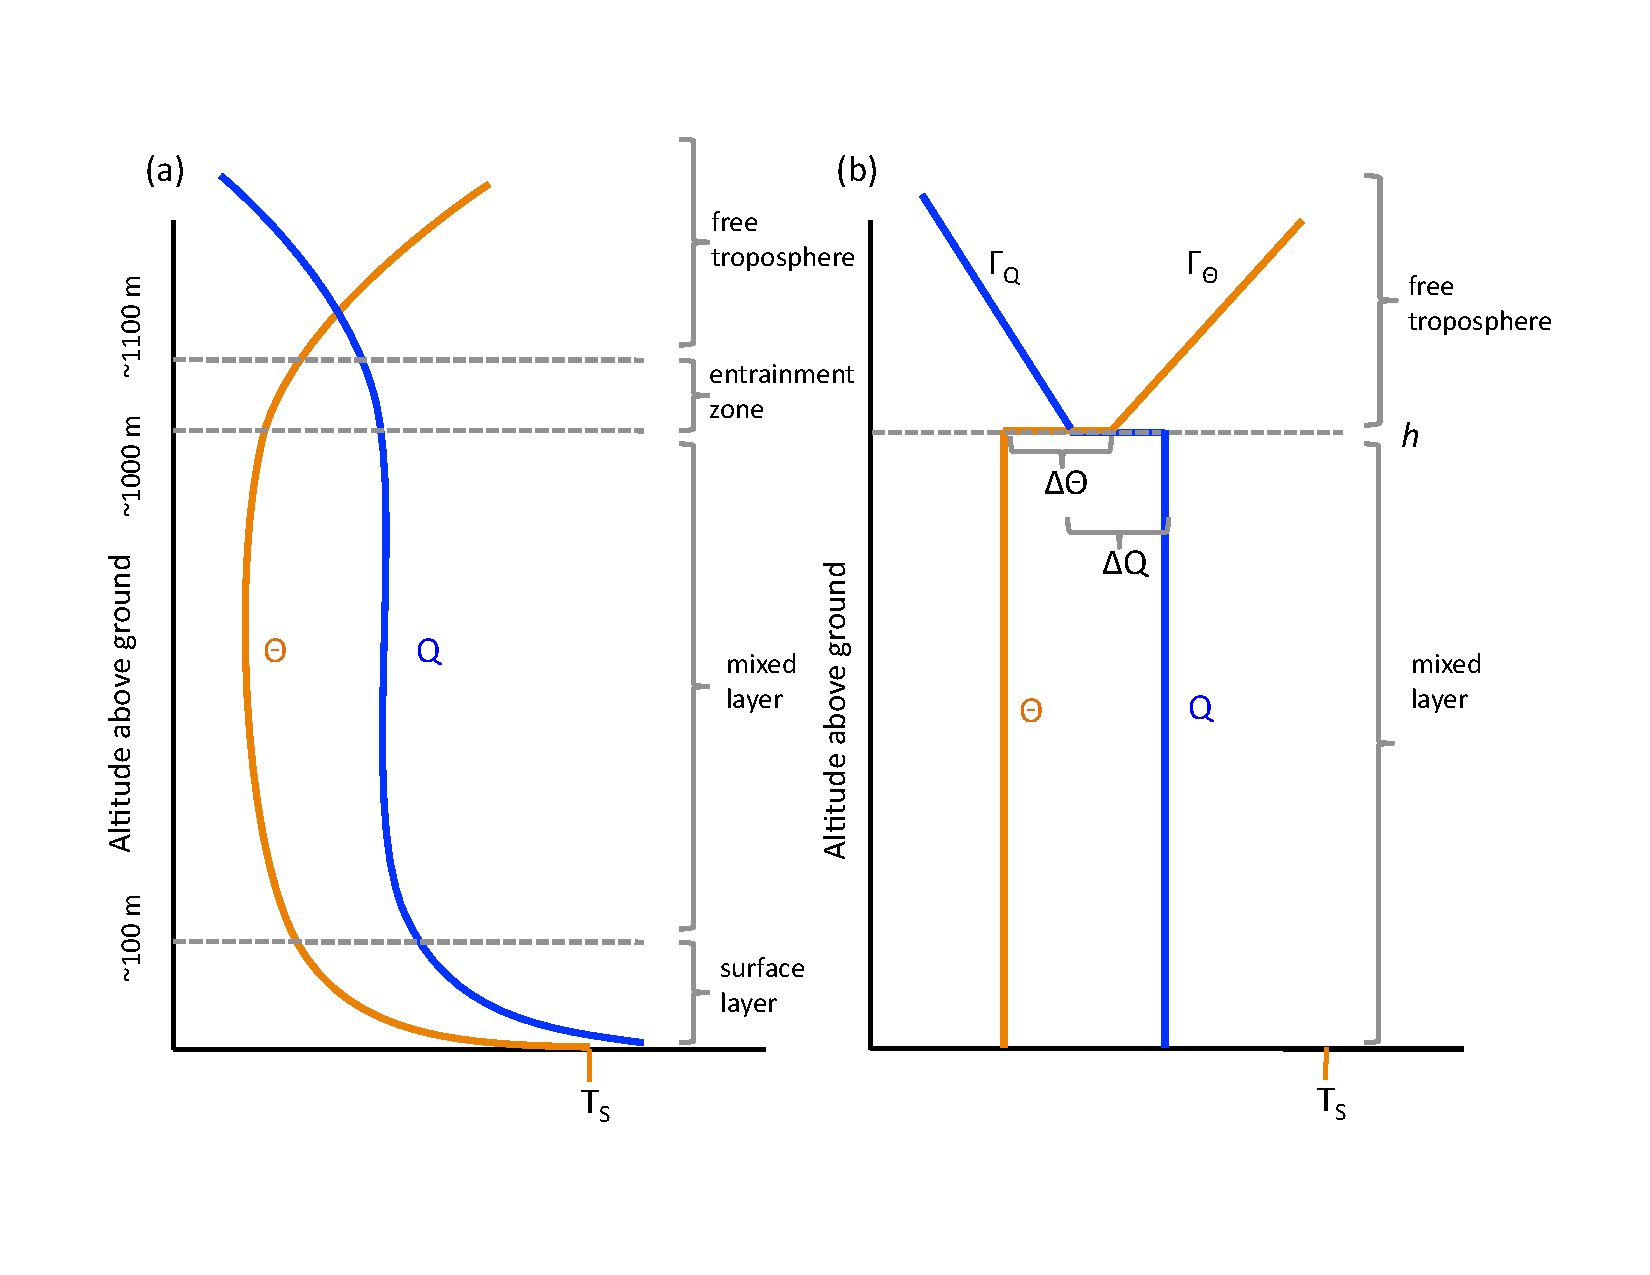
\includegraphics[width=1\textwidth]{ch2-BL/figures/schematic_mixed_layer.pdf}
\caption{(a) Schematic diagram of realistic potential temperature ($\Theta$, orange) and specific humidity ($Q$, blue) vertical profiles in a  daytime boundary layer.  (b) Vertical profiles of $\Theta$ and $Q$ in the 1-D model (adapted from Figure 2 from \cite{Siqueira:2009qf}).  $T_s$ represents the surface temperature.}
\label{fig:BL_schematic}
\end{figure}

\subsubsection{Model dynamics}
The height of the boundary layer, $h$ (m), is assumed in the 1-D to grow only by buoyant convection, in such a way that the entrainment heat flux at the top of the boundary layer is a fixed fraction of the sensible heat flux at the land surface (as in \cite{garratt1994atmospheric}, Section 6.1.5.)  The evolution of $h$ is modeled as

% dh/dt equation
\begin{equation}
\frac{dh}{dt} = (1+2\beta)\frac{H/\rho c_p}{\Gamma_\Theta h},
\label{eqn:dhdt}
\end{equation}
where $H$ is the surface sensible heat flux (W/m$^2$), $\rho$ is the density of air (kg/m$^3$), $c_p$ is the heat capacity of air at constant pressure (J/kg/K), $\Gamma_\Theta$ is the lapse rate of potential temperature above the boundary layer (K/m), and $1+2\beta$ is the proportionality relating surface sensible heat flux to entrainment heat flux at the top of the boundary layer; in this study, $\beta$ is set to 0.2, following \cite{garratt1994atmospheric}.  The time tendency of the boundary layer height, and thus of entrainment at the top of the boundary layer, is used to solve for the evolution of $\Theta$ and $Q$:

% dTheta/dt equation
\begin{equation}
\frac{d\Theta}{dt} = \frac{1}{h}\left(\frac{H}{\rho c_p}+\Delta\Theta\frac{dh}{dt}\right)
\label{eqn:dTdt}
\end{equation}
% dQ/dt equation
\begin{equation}
\frac{dQ}{dt} = \frac{1}{h}\left(\frac{E}{\rho}+\Delta Q \frac{dh}{dt}\right),
\label{eqn:dQdt}
\end{equation}
where $E$ is surface evapotranspiration (g/m$^2$/s), and $\Delta\Theta$ (K) and $\Delta Q$ (g/kg) are the jumps in potential temperature and specific humidity, respectively, across the inversion at the top of the mixed layer.  These jumps are calculated using

% dDTheta/dt equation
\begin{equation}
\frac{d\Delta\Theta}{dt} = \Gamma_\Theta\frac{dh}{dt}-\frac{d\Theta}{dt}
\label{eqn:dDTdt}
\end{equation}
% dDQ/dt equation
\begin{equation}
\frac{d\Delta Q}{dt} = \Gamma_Q\frac{dh}{dt}-\frac{dQ}{dt},
\label{eqn:dDQdt}
\end{equation}
where $\Gamma_Q$ is the lapse rate of water vapor above the mixed layer.  The first term on the right hand sides of Equations \ref{eqn:dQdt} and \ref{eqn:dDQdt} represents the rate of change in the value just above the inversion jump as the boundary layer grows, and the second term represents the rate of change in the mixed layer value; the difference between these two is the rate of change of the jump across the top of the mixed layer.

\subsubsection{External inputs and calculation of surface heat fluxes}
This model requires the following inputs: time series of evapotranspiration ($E$) and sensible heat flux ($H$) at the surface through the day; free tropospheric profiles $\Gamma_{\Theta}$ and $\Gamma_{Q}$; and initial conditions of $\Theta$, $Q$, $h$, $\Delta \Theta$, and $\Delta Q$.

$E$ is the sum of transpiration ($E_t$) and soil evaporation ($E_{soil}$); evaporation of intercepted canopy water is negligible during the dry season days considered here.  $E_t$ is simulated following the procedure in Section \ref{sec:sapflow_regmeth}: normalized sap velocity at the outer edge of the sapwood ($v_n$, ranging from 0 to 1) is predicted with a Jarvis model for stomatal conductance [\cite{jarvis1976interpretation}] with parameters estimated from sap flow measurements (species-averaged parameters in Table \ref{tbl:sapflow_maxvel}), and $v_n$ is scaled up to regional transpiration using the observed Douglas fir tree-diameter--sapwood-thickness relationship (Equation \ref{eqn:sapwood}) and an FIA-derived tree size distribution [\cite{woudenberg2010forest}, all-species distribution, black line in Figure \ref{fig:sapflow_abundances}].  The Douglas fir sapwood thickness relation is used for both the Douglas fir and Pacific madrone model runs because the relations are very similar and in order to eliminate variation due to sapwood area and focus on variation due to stomatal response.

Soil evaporation is estimated using a simplified version of the CLM model soil evaporation scheme [\cite{oleson2010technical}]:
\begin{equation}
E_{soil} = \frac{-\beta_{soi}(q_{air}-q_{ground})}{r_{aw}+r_{litter}},
\end{equation}
where $\beta_{soi}$ (unitless) is a reduction factor based on soil moisture (Equation 5.68 in \cite{oleson2010technical} with $\theta_{fc,1}=0.15$), $q_{air}$ is the specific humidity of the air (g/kg), $q_{ground}$ is the saturation specific humidity at ground temperature (g/kg), $r_{aw}$ (s/m) is the resistance to water vapor transfer from the ground to the canopy air space (Equation 5.99 in \cite{oleson2010technical} with $C_s=0.004$ (turbulent transfer coefficient, unitless) and $u_*=0.4$ m/s (friction velocity)), and $r_{litter}$ (s/m) is the resistance to water vapor transfer through the litter layer (Equation 5.106 in \cite{oleson2010technical} with $L^{eff}_{litter}=0.5$ m$^2$/m$^2$).  For the purpose of both $E_{soil}$ and $E_t$, soil moisture is treated as a single depth-averaged value, because the stomatal conductance parameters were fit with depth-averaged soil moisture, for reasons described in Sections \ref{sec:sapflow_sitedesc} and \ref{sec:sapflow_soilmoisture}.

Sensible heat flux ($H$, W/m$^2$) is calculated as
\begin{equation}
H = \frac{\rho c_p}{r_a} (T_s - T_a),
\end{equation} 
where the surface temperature ($T_s$, K) is determined by the evapotranspiration $E$ and the net radiation, and aerodynamic resistance ($r_a$) is held constant at 10 s/m.  This value of $r_a$ is representative of typical wind speeds and near-neutral conditions using Equation 14.33 from \cite{bonan}, and this particular value was chosen to give surface and air temperatures close to observations.  $T_s$ is derived by solving the surface energy balance equation,
\begin{equation}
(1-\alpha) S_{down} + L_{down} - \sigma \epsilon T_s^4 = \frac{\rho c_p}{r_a} (T_s - T_a) + \lambda E + G
\label{eqn:seb}
\end{equation}
where $\alpha$ is surface albedo (unitless), $S_{down}$ is downward solar radiation (W/m$^2$), $L_{down}$ is downward longwave radiation (W/m$^2$), the last term on the left hand side is outgoing longwave radiation ($L_{up}$, W/m$^2$), $\sigma$ is the Stefan-Boltzmann constant (W/m$^2$/K$^4$), $\epsilon$ is surface emissivity (unitless), the first term on the right hand side is $H$, $\lambda$ is the latent heat of vaporization of water (J/g/K), and the ground heat flux $G$ is set equal to 10\% of the net radiation (sum of the left-hand-side terms) [\cite{ogee2001long}].  Equation \ref{eqn:seb} is solved for $T_s$ using the Newton-Raphson method and a timestep of 1 second.  $H$ for input to the 1-D model is then calculated using $T_s$, modeled $\Theta$ converted to $T_a$, and the fixed value of $r_a$.  The modeled potential temperature $\Theta$ is converted to near-surface air temperature $T_a$ (needed for calculating $H$ and $E_t$, which requires VPD) by adjusting for the ground-surface elevation at the ACRR, using an altitude at ground level of 400 m above sea level (ASL) and an adiabatic lapse rate of 10 K/km ($\Theta = T_a$(0 m ASL); $T_a$(400 m ASL) $= T_a$(0 m ASL) - (10 K/km)(0.4 km)).

Incoming radiation is prescribed using typical values for August in this region.  For $S_{down}$, we use the average diurnal course of total solar radiation measured at an open meadow station at the Angelo Coast Range Reserve (ACRR) on August 15 of 2009-2011, as representative of clear days in mid-August, when soil moisture has dried enough to begin to limit transpiration.  For $L_{down}$, we use the GEWEX Surface Radiation Budget [\cite{stackhouse2011nasa}] mean diurnal pattern from the month of August (using the years available, 2003-2007) for the grid cell nearest the ACRR field site.  $\alpha$ is set to 0.1 and $\epsilon$ is set to 0.95 for both species in order to eliminate variation due to vegetation radiative properties (0.1 is the albedo and 0.95 is the emissivity for broadleaf evergreen temperate trees in CLM [\cite{oleson2010technical}].)

Free troposphere conditions (needed for $\Gamma_{\Theta}$ and $\Gamma_Q$ in Equations \ref{eqn:dhdt}, \ref{eqn:dDTdt}, and \ref{eqn:dDQdt}) are derived from atmospheric soundings at Oakland International Airport, 250 km south of the Rivendell field site (downloaded from the archive at the University of Wyoming, \url{http://weather.uwyo.edu/upperair/sounding.html}).  The sounding site and field site are similar distances from the Pacific coast (16 km for the field site and 25 km for Oakland Airport) and both have prevailing wind directions from the west over the ocean.  As such, the pre-dawn free troposphere profiles have minimal land-surface influence and instead sample the background air mass, which in the long term average is likely to be fairly uniform across a distance of 250 km (less than the Rossby radius of deformation).  Oakland is influenced by fog, but it is also at lower altitude (near sea level), whereas much of northern Coast Range forest region has a base elevation of at least 400 m ASL; as such, we neglect sounding measurements from below 400 m ASL, thus excluding much of the fog.  Profiles of $\Theta$ and $Q$ are available for 4 AM and 4 PM local time; here, we average profiles from 4 AM local time for the months of July and August from 2009 to 2011, binned by daily maximum temperature ($T_{max}$) measured at the ACRR: cool days ($T_{max} < 20^{\circ}$C), intermediate days ($20^{\circ}$C $\le T_{max} < 30^{\circ}$C), and hot days ($T_{max} \ge 30^{\circ}$C).  We use $T_{max}$ at Angelo as an indicator of warmer versus colder free troposphere conditions, because given similar radiation conditions, day-to-day temperature variation is driven largely by variation in the free troposphere air masses.  The average profiles and the piecewise linear approximations used in the model are shown in Figure \ref{fig:BL_LapseRates}.

\begin{figure}[here]
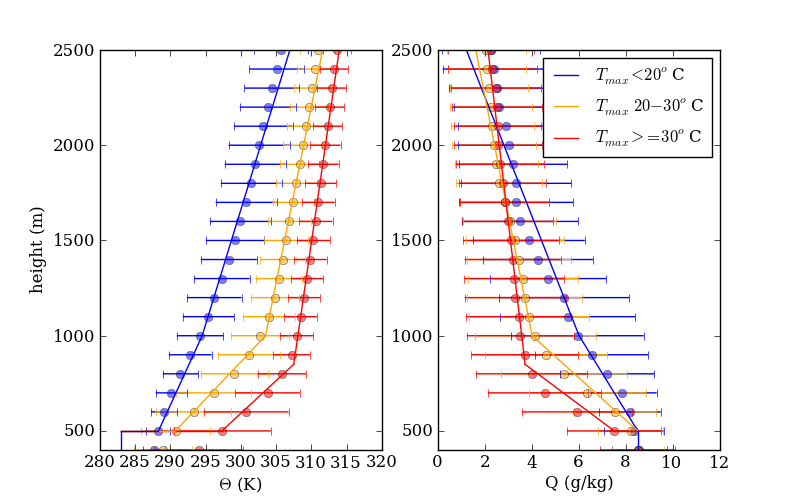
\includegraphics[width=1\textwidth]{ch2-BL/figures/fitted_lapserates_theta_Q_onefig.png}
\caption{Symbols: potential temperature ($\Theta$, left) and specific humidity ($Q$, right) from Oakland Airport soundings at 04:00 local time, averaged for July and August 2009-2011 and binned by height.  Error bars show one standard deviation.  Lines: piecewise linear approximations to the lapse rates for $\Theta$ and $Q$, which are used in the 1-D boundary layer model.}
\label{fig:BL_LapseRates}
\end{figure}

The model is initialized at 7:45 AM local time with boundary layer depth $h=$ 100 m as a rough estimate of nocturnal boundary layer depth over complex terrain, and with $\Theta=$ 283 K and $Q=$ 8.5 g/kg, based on average early morning values measured at the ACRR in August.  The model is not very sensitive to initial conditions, instead adjusting quickly to the daytime radiation and surface energy constraints (not shown).

The range of soil moisture, free troposphere, and tree species conditions tested are listed in Table \ref{table:BL_1Druns}.  

\begin{table}
\begin{tabular}{ p{7.5cm} p{7.5cm} }
\hline
Parameter & Range of values tested \\ \hline
Jarvis $VPD$ parameters ($D_o$ and $g_{c,max}$) and $\theta_{rel}$ parameters ($\theta_0$ and $\beta$) & Douglas fir, Pacific madrone (Table \ref{tbl:sapflow_mcmc}, species-averaged values)\\
Lapse rates $\Gamma_{\Theta}$ and $\Gamma_Q$ & 1 (blue in Figure \ref{fig:BL_LapseRates}), 2 (yellow), 3 (red)\\
Relative soil moisture $\theta_{rel} $ (unitless) & 0.15, 0.2, 0.25, 0.3, 0.35, 0.4, 0.45, 0.5\\
\hline
\end{tabular}
\caption{Range of values tested using the one-dimensional boundary layer model.}
\label{table:BL_1Druns}
\end{table}

\subsection{Regional climate model}
\label{sec:BL_WRFdesc}
In order to further test the impact of these two tree species on the atmospheric boundary layer, we use WRF-Noah [\cite{skamarock2008}], a three-dimensional, non-hydrostatic regional climate model (Weather Research and Forecasting, or WRF) with terrain-following vertical coordinates and a coupled land surface model (Noah).  In WRF, the conservation equations for momentum, mass, and energy are solved numerically to calculate the temporal evolution of atmospheric state variables, including air temperature, pressure, humidity, and wind velocity.  WRF has a range of parameterization options for radiation, turbulence treatment via planetary boundary layer (PBL) schemes or large-eddy simulation closures, cloud microphysics, convection, bottom boundary fluxes of water vapor and heat, and lateral boundary forcing.  

\begin{table}
\begin{tabular}{l l}
\hline
Scheme & Setting \\ \hline
WRF version & 3.6 \\
Grid nesting & two-way \\
Lateral boundary conditions & NCEP Eta analysis \\
Soil levels & 4 \\
Land use and soil categories & USGS \\
Land surface model & Noah \\
Surface layer & MM5 Monin-Obukhov \\
Planetary Boundary Layer (PBL) & ACM2 \\
Turbulence closure & Horizontal Smagorinzky first order \\
Microphysics & WSM 3-class simple ice \\
Longwave radiation & RRTM \\
Shortwave radiation & Dudhia \\
Cumulus & Kain-Fritsch (new Eta) \\
Momentum advection & 5th order horizontal, 3rd order vertical \\
Scalar advection & 5th order positive definite \\
Lateral boundary relaxation zone & 5 grid points \\
\hline
\end{tabular}
\caption{WRF parameterization options.  See \cite{skamarock2008} for description of schemes.}
\label{table:BL_paramschemes}
\end{table}

The parameterization schemes used here are listed in Table \ref{table:BL_paramschemes}.  Most schemes chosen are the default settings for realistic (non-idealized) simulations, with the exception of the ACM2 PBL scheme. The ACM2 scheme is used because of its ability to represent both convective regimes (non-local transport) and shear-dominated regimes (local transport) [\cite{pleim2007combined}], and because of its good performance in other WRF studies [\cite{xie2012evaluation}, \cite{xie2013structure}, \cite{deppe2013wrf}, \cite{marjanovic2014}].

\begin{table}
\begin{tabular}{ l c c c c c c c }
\hline
Domain & $\Delta x$ (km) & $\Delta y$ (km) & $nx$ & $ny$ & $nz$ & $\Delta t$ (s) & USGS data res \\ \hline
d01 & 8.1 & 8.1 & 96 & 99 & 45 & 45 & 2 min\\
d02 & 2.7 & 2.7 & 175 & 175 & 45 & 15 & 2 min\\
\hline
\end{tabular}
\caption{Model domains. d01 refers to the outer domain, and d02 refers to the inner domain.}
\label{table:BL_domains}
\end{table}

\begin{figure}[here]
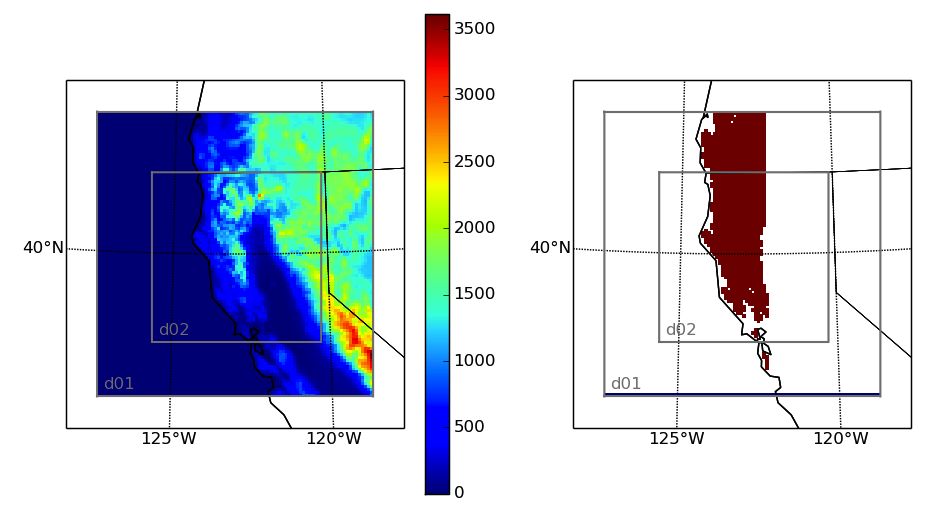
\includegraphics[width=1\textwidth]{ch2-BL/figures/domain_map_cropped.png}
\caption{WRF domains over northern California.  The gray outlines show the domain boundaries; d01 is the outer nest, and d02 is the inner nest.  Left: topographic elevation (m); right: red shows the test region where vegetation parameters are modified.}
\label{fig:BL_domain}
\end{figure}

The tests are run with two nested domains centered on the northern Coast Range (Figure \ref{fig:BL_domain}).  The use of two nests enables gradual down-scaling of the coarse lateral forcing to the high resolution needed to better resolve flow over the Coast Range.  We adopt a conservative nesting grid ratio of 3:1.  The outer domain (``d01'') provides the lateral boundary conditions for the inner domain (``d02''), and the inner domain states are fed back to the outer domain throughout the region coincident with the inner domain.  Two-way nesting increases model accuracy, particularly in regions of complex terrain [\cite{harris2010idealized}, \cite{marjanovic2014}].  The domain resolutions and dimensions are listed in Table \ref{table:BL_domains}.  The lateral boundaries of the outer domain are forced with NCEP Eta 212 grid (40 km) operational analysis [\cite{ncep}] for the period of 2009-08-16 00:00 to 2009-08-30 00:00, with the first 32 hours discarded as model spin-up.  This time period is rain-free and sunny at the Angelo Reserve and represents the mid- to late-summer season when soil is very dry and incoming radiation is still strong (Figure \ref{fig:sapflow_met}).

The two hypothetical forests (all-Douglas-fir and all-Pacific-madrone) are tested in the northern Coast Range region highlighted in Figure \ref{fig:BL_domain}.  In this region, idealized land use and soil types are used, and the VPD and soil moisture stomatal response parameters of this dummy type are modified according to the test case, as described below.  Radiative properties, leaf area, and rooting depth of the dummy type are held constant among the test cases, using the ``Evergreen Needleleaf Forest'' values.  Outside of the test region, observed topography and USGS classification system vegetation and soil types are used [\cite{skamarock2008}].

\begin{table}
\begin{tabular}{ l p{3cm} p{3cm} p{2cm} p{3cm} }
\hline
Vegetation type & $\theta_{ref}$ (m$^3$/m$^3$) & $\theta_{wilt}$ (m$^3$/m$^3$) & $RS$ (s/m) & $HS$ (kg/kg)\\ \hline
%ENF & 0.329 (loam) & 0.066 (loam) & 125 & 47.35\\
Douglas fir & 0.156 & 0.075 & 125 (ENF) & 47.35 (ENF)\\
%EBF & 0.329 (loam) & 0.066 (loam) & 150 & 41.69\\
Pacific madrone & 0.105 & 0.047 & 150 (EBF) & 41.69 (EBF)\\
%Pacific madrone 2 & 0.105 & 0.047 & 300 & 20.\\
\hline
\end{tabular}
\caption{Parameters for Noah's Jarvis formulation of stomatal conductance, by vegetation type.  $\theta_{ref}$ and $\theta_{wilt}$ are the volumetric soil moisture values defined in Equation \ref{eqn:f_theta} and Figure \ref{fig:BL_FeddesParams}.  $RS$ is the Noah minimum stomatal resistance parameter in the Jarvis formulation. $HS$ is the Noah scaling factor for the specific humidity deficit in the Jarvis humidity stress function (Equation \ref{eqn:BL_WRFq}).  ENF is the USGS Evergreen Needleleaf Forest land use type; EBF is the USGS Evergreen Broadleaf Forest land use type.}
\label{table:BL_NoahJarvisparams}
\end{table}

\begin{table}
\begin{tabular}{ l p{6cm} p{7cm} }
\hline
Run ID & VPD parameters ($RS$, $HS$) & Soil moisture parameters ($\theta_{ref}$, $\theta_{wilt}$)\\ \hline
vDF-sDF & Douglas fir (ENF) & Douglas fir\\
%vEBF-sMD & EBF & Pacific madrone\\
vMD-sMD & Pacific madrone (EBF) & Pacific madrone\\
%vMD2-sMD & Pacific madrone 2 & Pacific madrone\\
\hline
\end{tabular}
\caption{Combinations of stomatal conductance Jarvis parameters used in the WRF tests.  Each pair of parameters is tested for a range of volumetric soil moisture ($\theta_{vol}$) values in the northern Coast Range test region: 0.08, 0.1, 0.12, and 0.14 m$^3$/m$^3$ (equivalent to $\theta_{rel}$ of 0.18, 0.23, 0.27, and 0.32 with $\theta_{max} = 0.439$ m$^3$/m$^3$.}
\label{table:BL_WRFruns}
\end{table}

The test region stomatal conductance parameters are modified to quantify the differences between the hypothetical all-Douglas-fir and all-Pacific-madrone cases.  The Noah model uses a Jarvis formulation of stomatal conductance similar to that used in Chapter \ref{c.sapflow} (Equation \ref{eqn:sapflow_jarvis_simple}):
\begin{equation}
\frac{1}{r_c} = \frac{1}{RS} f_{\theta} f_{\Delta q} f_{rad} ...
\end{equation}
The $RS$ parameter is the minimum stomatal resistance (equivalent to $1/g_{s,max}$), and the maximum stomatal conductance $\frac{1}{RS}$ is modified by empirical functions of environmental variables ($f_{\theta}$, $f_{\Delta q}$, $f_{rad}$) to give the actual stomatal conductance (inverse stomatal resistance) $\frac{1}{r_c}$.  

The soil moisture stress function is the piecewise-linear, threshold Feddes model [\cite{feddes}; \cite{chen2008observations}]:
\stepcounter{equation}
\begin{displaymath}
   f_{\theta}(\theta) = \left\{
     \begin{array}{lr}
       1 & : \theta > \theta_{ref}\\
       \frac{\theta - \theta_{wilt}}{\theta_{ref} - \theta_{wilt}} & : \theta_{wilt} < \theta \leq \theta_{ref} \tag{\theequation}\\
       0 & : \theta \leq \theta_{wilt}
     \end{array}
   \right.
   \label{eqn:f_theta}
\end{displaymath} 
%\begin{equation}
%f_{\theta} = \frac{\theta - \theta_{wilt}}{.
%\end{equation}
The parameters for the sigmoid model from Chapter \ref{c.sapflow} (Equation \ref{eqn:sapflow_soilmois}, Table \ref{tbl:sapflow_mcmc}) thus must be translated to the Feddes parameters (reference or stress point, $\theta_{ref}$, and wilting point, $\theta_{wilt}$).  For each species, we fit a line to $f_{\theta}$ between $f_{\theta}=0.05$ and $f_{\theta}=0.95$ and extrapolate the line to 0 to estimate $\theta_{wilt}$ and to 1 to estimate $\theta_{ref}$ (Figure \ref{fig:BL_FeddesParams}, Table \ref{table:BL_NoahJarvisparams} where $\theta_{rel}$ values are converted to $\theta_{volumetric}$ using $\theta_{max} = 0.439$ m$^3$/m$^3$ for the dominant loam soil type in the test region).

%atmospheric effects of the two tree species are tested by modifying the stomatal conductance parameters for the dummy vegetation and soil types in the test region.

The empirical function representing humidity stress in the Noah model is similar to the asymptotic function used in Chapter \ref{c.sapflow} (Equation \ref{eqn:sapflow_fVPD}):

\begin{equation}
f_{\Delta q}(\Delta q) = \frac{1}{1+HS \Delta q},
\label{eqn:BL_WRFq}
\end{equation}
where $\Delta q$ (kg/kg) is the difference between saturated specific humidity and actual specific humidity, and $HS$ relates changes in humidity to changes in stomatal conductance (analogous to $D_o$ in Chapter \ref{c.sapflow}), with values given in Table \ref{table:BL_NoahJarvisparams}.

\begin{figure}[here]
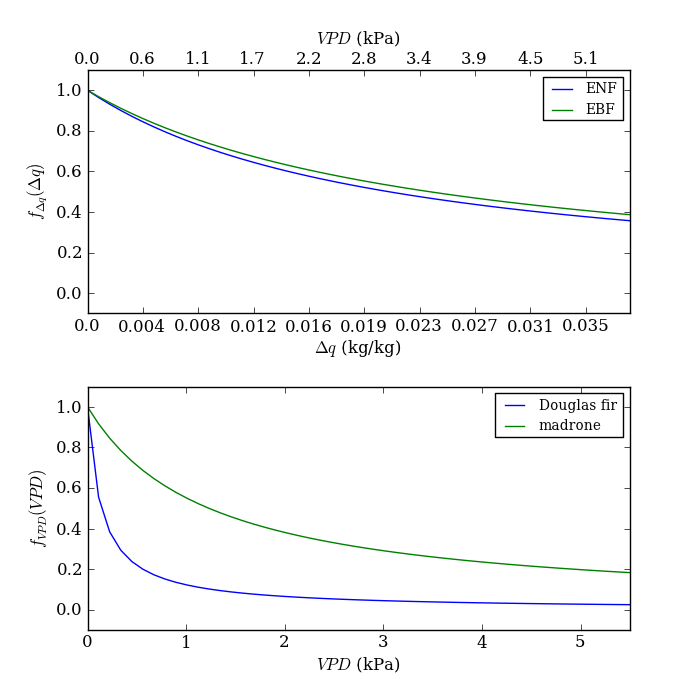
\includegraphics[width=0.9\textwidth]{ch2-BL/figures/humidity_functions.png}
\caption{Jarvis humidity function using WRF Noah parameters for EBF and ENF (top panel), compared to the Jarvis function using sap-flow-derived parameters (bottom panel).  The WRF Noah humidity function is based on specific humidity deficit ($\Delta q$, top panel bottom axis); in the top panel, $\Delta q$ was converted to $VPD$ for comparison with the bottom panel, assuming an air temperature of 35$^\circ$C and air pressure of 900 hPa.}
\label{fig:BL_humidity}
\end{figure}

The variation of $f_{\Delta q}$ with $\Delta q$, using USGS $HS$ parameters for Evergreen Needleleaf Forest (ENF, blue) and Evergreen Broadleaf Forest (EBF, green), is shown in Figure \ref{fig:BL_humidity} (top panel).  For comparison, the variation of $g_{s, max}/\alpha * f(VPD)$ with $VPD$, calculated using sap-flow-derived species averaged parameters for Douglas fir and Pacific madrone (Table \ref{tbl:sapflow_mcmc}), is also shown in Figure \ref{fig:BL_humidity} (bottom panel).  In the sap-flow-derived parameters, the Douglas-fir case has higher stomatal conductance at low $VPD$, whereas the difference is much less pronounced at low $VPD$ in the WRF parameters.  Despite these differences, for the tests presented here, we use the Noah ENF and EBF parameters to represent the species difference in humidity response.  We do not use the sap-flow-derived parameters for several reasons: (1) it is not straightforward to translate the sap-flow-based $g_{s,max}/\alpha$ to $RS$, because $g_{s,max}/\alpha$ refers to stomatal conductance normalized by sapwood area, whereas $RS$ represents resistance on a per-unit-leaf-area basis; (2) $D_o$ is in units of $VPD$ (kPa), while $HS$ is in units of inverse specific humidity ($q$, kg/kg), and the relation between $VPD$ and $q$ varies with temperature; and (3) the atmospheric boundary layer effects when soils are dry depend much more on species differences in soil moisture response than on species differences in humidity response (Figure \ref{fig:BL_testVPDtheta}, below); as such, the impact of errors in humidity response parameters on results from hot summer days is expected to be small.

\begin{figure}[here]
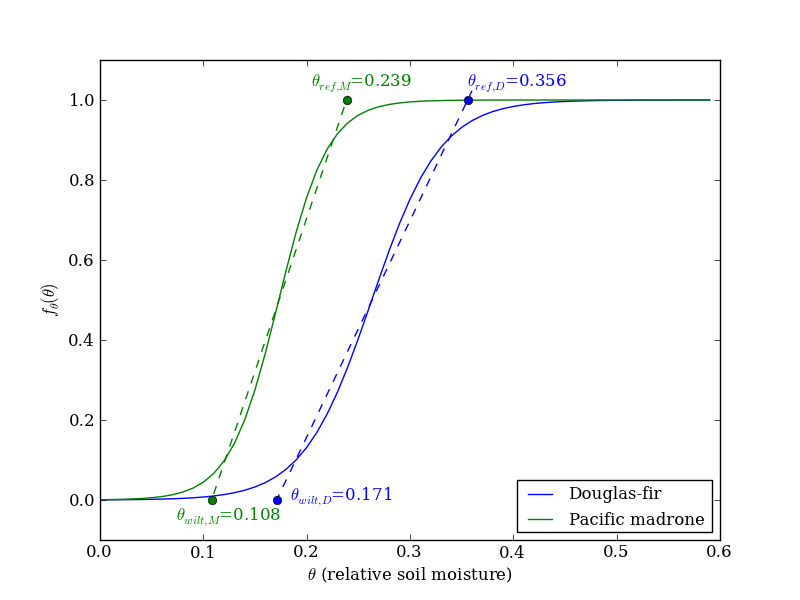
\includegraphics[width=0.9\textwidth]{ch2-BL/figures/theta_params.png}
\caption{Solid lines: sigmoid $f_{\theta}$ functions (Equation \ref{eqn:sapflow_soilmois}) for Douglas fir (blue) and Pacific madrone (green) using the species-averaged parameters from Table \ref{tbl:sapflow_mcmc}.  Dashed lines: linear regression to $f_{\theta}$ between 0.05 and 0.95.  Symbols: extrapolation of linear regression to $f_{\theta}=0$ and $1$.}
\label{fig:BL_FeddesParams}
\end{figure}

WRF-Noah is run for the all-Douglas-fir and all-Pacific-madrone cases (Tables \ref{table:BL_NoahJarvisparams} and \ref{table:BL_WRFruns}), with a range of volumetric soil moisture values ($\theta_{vol} =$ 0.08, 0.1, 0.12, 0.14 m$^3$/m$^3$).  These values are equivalent to relative soil moistures of 0.18, 0.23, 0.27, and 0.32, given that the saturation moisture content of the loam soil type used in the model is 0.439 m$^3$/m$^3$.  These relative soil moisture values span the range of values observed in August at the Angelo Coast Range Reserve (Figure \ref{fig:sapflow_met}).  Soil moisture in the Coast Range test region is reset each day at midnight local time, so that the soil moisture deviates only minimally from its stated value (less than 10\%).

WRF results are presented at two elevations: 2 m above ground level (AGL), which is in the surface layer (Figure \ref{fig:BL_schematic}), and 390 m AGL, which is in the mixed layer of the fully-developed inland boundary layer.
